%证明闭合曲面的法向量面积分为零
% 多元微积分|矢量积分|体积分|闭合曲面|散度|散度定理|通量

%(未完成)
\pentry{散度 散度定理\upref{Divgnc}}

对于闭合曲面 $\Omega$,  证明 $\oint_\Omega  \dd{\bvec s} = \bvec 0$, 其中 $\dd{\bvec s}$ 是曲面上的面元矢量,其模长 $\dd{s}$ 为面元的面积,  方向为沿着该面元的法线向外.
把矢量积分分解成三个分量,有
\begin{equation}
\begin{aligned}
\oint_\Omega  \dd{\bvec s} & = \oint_\Omega  [(\uvec x \dd{\bvec s})\uvec x + (\uvec y \dd{\bvec s})\uvec y + (\uvec z \dd{\bvec s})\uvec z] \\
&= \uvec x\oint_\Omega  \uvec x \dd{\bvec s}  + \uvec y\oint_\Omega \uvec y \dd{\bvec s} + \uvec z\oint\limits_\Omega \uvec z \dd{\bvec s}
\end{aligned}
\end{equation}
下面以第一项为例,证明积分结果为 0, 后两项的证明类似.
根据散度定理,矢量场在闭合曲面上的通量等于该矢量场散度在曲面内空间的体积分,所以
\begin{equation}
\oint_\Omega  \uvec x \dd{\bvec s}  = \int_V (\div \uvec x) \dd{V}  = \int_V 0 \dd{V}  = 0
\end{equation}
\begin{figure}[ht]
\centering
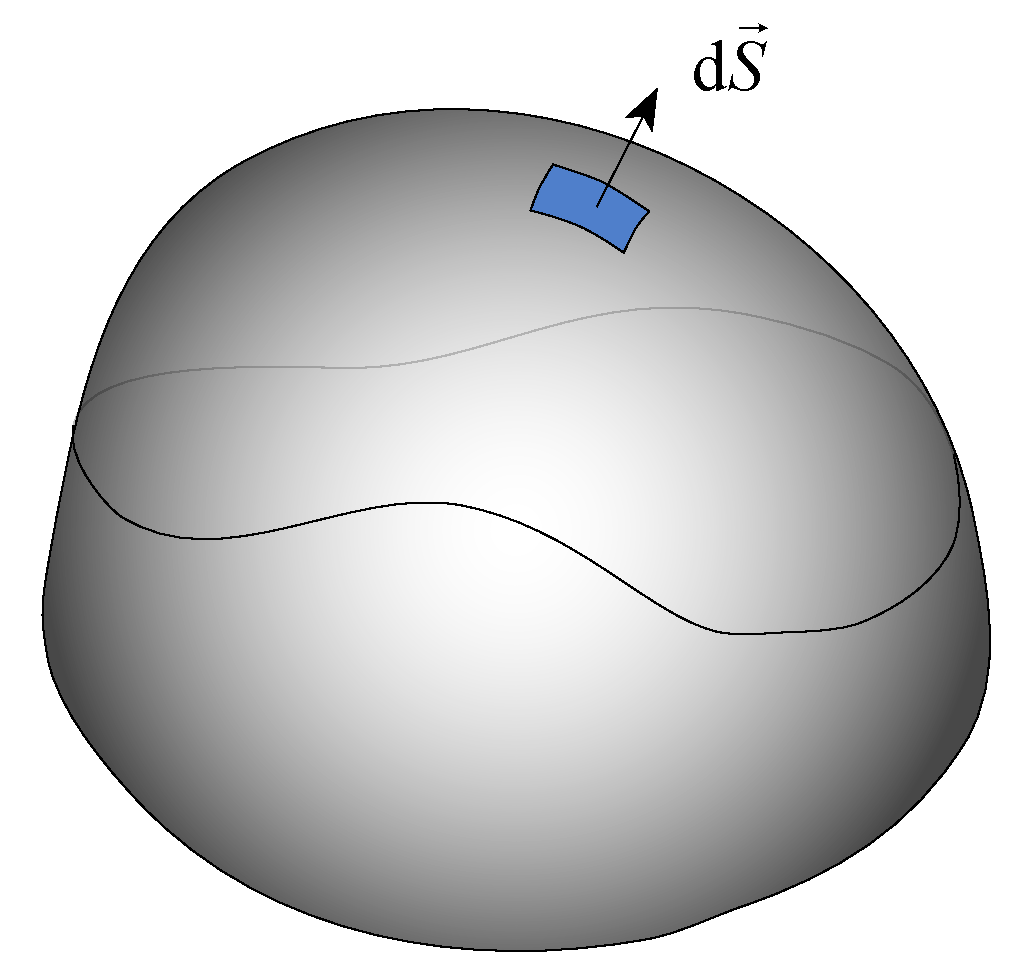
\includegraphics[width=5.34cm]{./figures/CSI0_1.pdf}
\caption{闭合曲面上的一个面元} \label{CSI0_fig1}
\end{figure}

 
 

